\documentclass[titlepage]{article}

\usepackage{amssymb,amsmath,amsthm}
\usepackage{graphicx} % Package for including figures
%\usepackage{psfrag,color}
\usepackage[utf8]{inputenc}
\usepackage{longtable}

\title{HW3 Data Report for Math/CS 471}
\author{AUTHOR1}
\date{10/01/2017}   % Activate to display a given date or no date


\begin{document}
\maketitle

\begin{abstract}
This is the HW3 report. This report is made all through LaTeX. This
report's data was produced by Fortran 90 and the plots were produced
by matlab. Finally, the author used Perl to run Latex, write
discussion, and incorporate the four plots.
\end{abstract}

\section{Problem Description}
In this assignment, an integral is given with two different efficients
(k=pi and k=pi*pi). The author will use two different computing methods
to approximate the value of intergral I. The language for computing is
Fortran. The knowledge will cover Trapezoidal rule as well as Gauss
Quadrature. Others like Makefile and MATLAB plotting will also be
used. The author wants to find out when the error: abs(theoretical value -
approximate value) will be smaller than $10^{-10}$ and how many
iterarions (n) will be used for this convergence. It is worth noting
that for Trapezoidal rule both cases coverge at last and they all stop
before my iteration upper limit (n=100000 times). However, they didn't converge
as small as  $10^{-10}$ in Gauss Quadrature. The best error is about
$10^{-8}$. The theoretical values for both k = pi and k = pi* pi are
from Trapezoidal rule when the author set the equidistant grids be
$10^{8}$, which should be able to give a good approximation close to
theoretical value. All of them all start with n = 2 and XL = -1 and XR = 1.

\section{Method 1: Trapezoidal rule}
\subsection{introduction}
Trapezoidal rule approximates the integrals using equiditant
grids. The order for this method is 2 in Trapezoidal rule. The author
uses Fortran to write a program for composite trapezoidal and try to
find the value which is more closer to the theoretical value of this
integral. The N I used is 10$^8$ which should be accurate enough for
giving a good theoretical value. Then the author will use different numbers of
equidistant grids (n) to find different approximate integral values
and plot their absolute value of error: abs(theoretical value -
approximate value) corresponding to n's values. Both k=pi and k=pi*pi
will be in the same picture.

\subsection{Figures1}
\subsubsection{Question 1} 
Question: Plot the error against n using a logarithmic scale for both axes.\\
Ans: Fig1 is the figure for the Trapezoidal rule plot. I plot all the n
whoses error is bigger than $10^{-10}$. My n starts from 2 and XL = -1
and XR = 1. Both x axis plot and y axis plot are logarithmic scale.

\begin{figure}[htb]
\begin{center}
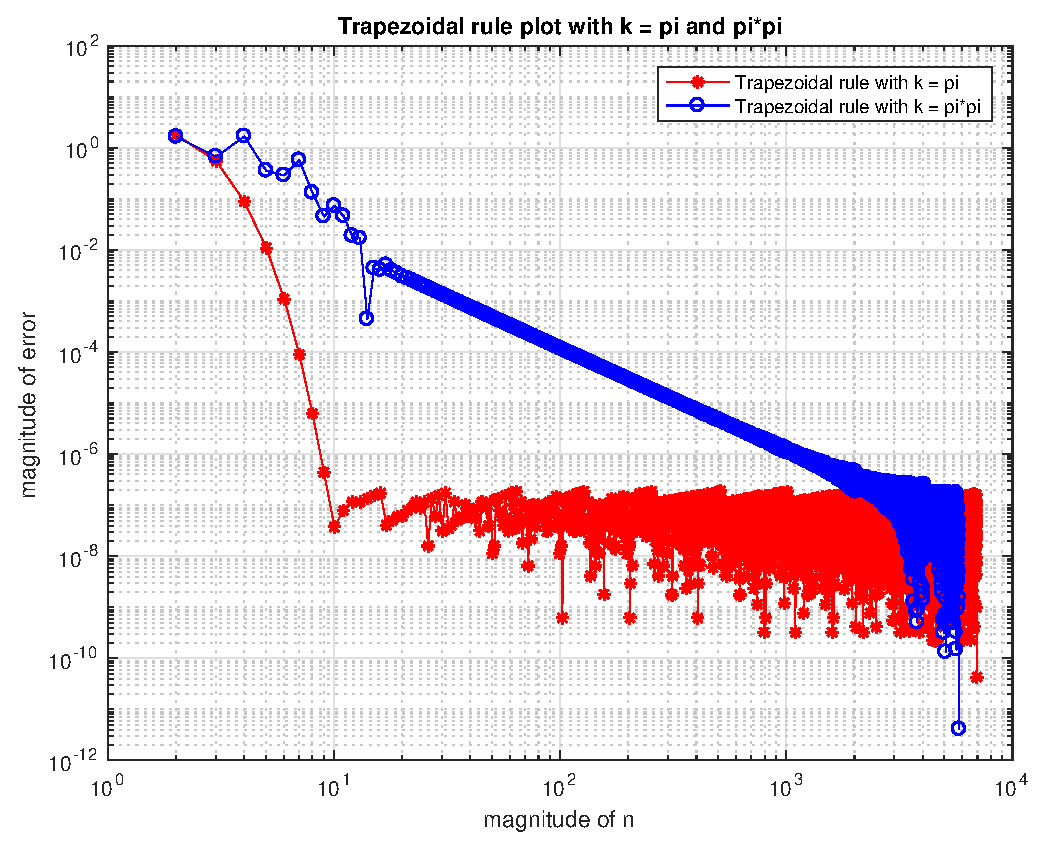
\includegraphics[width=1.0\textwidth]{Trapezoidal.eps}
\caption{Trapezoidal rule plot with k = pi and pi*pi. \label{fig:1}}
\end{center}
\end{figure}

\subsubsection{Question 2}
Question: Read off the order of the method from the slopes and theory discussion.\\
Ans: Yes, actually based on the plots and the shape of the curve, I
find the slope with k=pi is much larger than that with
k=pi*pi. Trapezoidal rule with k = pi converges faster. From the
perspective of theory, remember when Professor derived the Trapezoidal
rule, there is a Trap Error which includes a term: $f(x)^"$. (just in
case, it is f(x) double prime) This term
is required to be bonded with XL and XR. When the coefficient k is
much lager (pi*pi > pi) the results got from $f(x)^"$ would be much
larger because when you differentiate it twice, the coefficients go
outside. At this moment the curve will become flat, therefore, it comes to
theoretical value slower (Big Trap Error slowers the curve and makes
it flat).
\subsubsection{Question 3} 
Question: Why k = pi converges faster and what is special with k=pi?\\
Ans: The Euler–Maclaurin formula according to WiKi is used for detailed
error analysis in numerical quadrature, which explains the superior
performance of the trapezoidal rule on smooth periodic functions. In
the equation $S - I = \sum\limits_{k=1}^p Bk/k! * (f(XR)^{k-1} -
f(XL)^{k-1}) + R$. S is the sum and I is the Integral value. Bk is the
kth Bernoulli number and R is an error term. Smaller cofficient k=pi
leads to smaller (S-I) value when the differentiation happens, which makes
the approimation converge faster. 
\subsection{Trapezoidal rule results discussion}
Using Trapezoidal rule the author got the Fig.1 data plot. Luckily,
both of them finally convege. Besides they all make the error smaller
than $10^{-10}$ before n comes to $10^5$. The case where coefficient
k = pi converges faster than that where k = pi*pi. 


\section{Method 2: Gauss Quadrature}
\subsection{introduction}
In this part, Gauss Quadrature method is used to approximate the
results of this integral. The author uses Fortran to call a subroutine
and tries to find the value which is more close to the theoretical value of this
integral. The N I used is 10$^8$ which should be accurate enough for
giving a good theoretical value. The theoretical value is from Trapezoidal rule 
with n = 10$^8$. Then the author will use different numbers of
n (number of Gauss points) to find different approximate integral values
and plot their absolute value of error: abs(theoretical value -
approximate value) corresponding to n's values. Both k=pi and k=pi*pi
will be in the same picture.
\subsection{Figures2}
\subsubsection{Question 1} 
Question: Plot the error against n using a logarithmic scale for both axes.\\
Ans: Fig2 is the figure for the Gauss Quadrature plot. I plot all the
first 5000 n's error. Almost all of them have the error larger than
$10^{-8}$. My n starts from 2 and XL = -1 and XR = 1. Both x axis plot
and y axis plot are logarithmic scale. 

\begin{figure}[htb]
\begin{center}
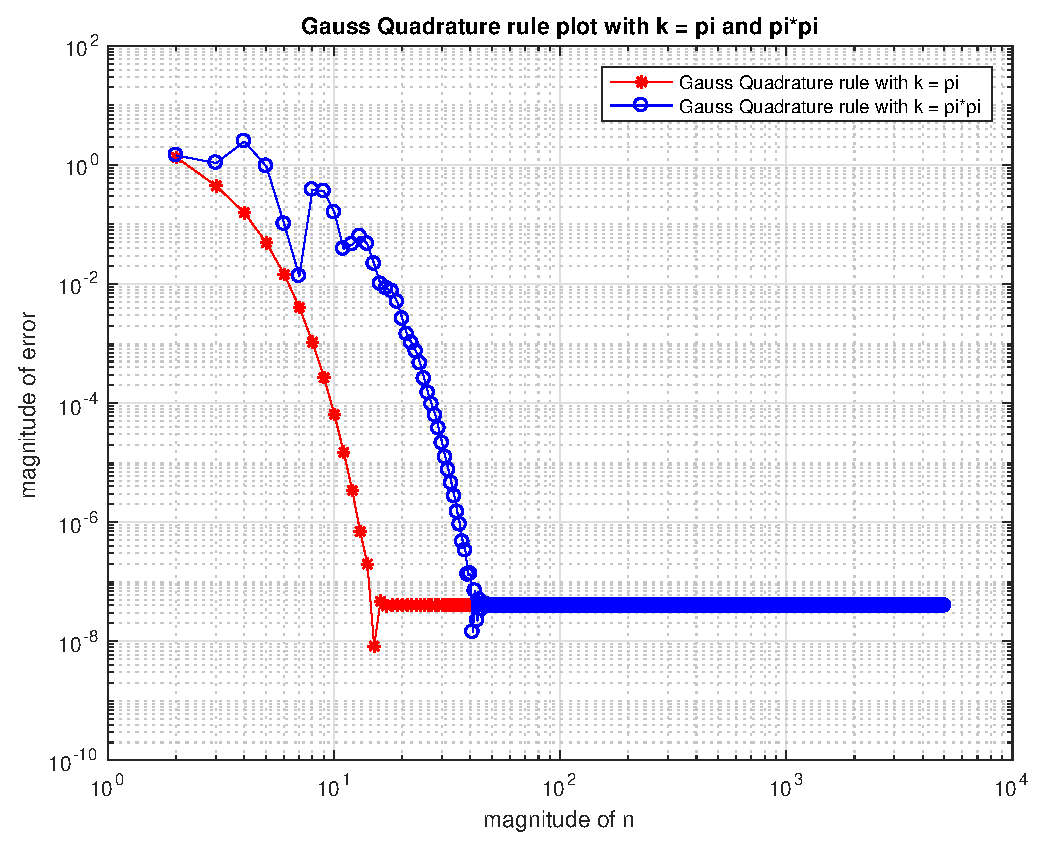
\includegraphics[width=1.0\textwidth]{Gauss.eps}
\caption{Gauss Quadrature rule plot with k = pi and pi*pi. \label{fig:2}}
\end{center}
\end{figure} 

\subsubsection{Question 2}
Question: Try some different C and a to get a good $C^{-an}$ plot fitting the
curves.\\
Ans: For the case k = pi, the author chooses C = 1000 and a = 0.1.\\
For the case k = pi*pi, the author chooses C = 70 and a = 0.09.
\begin{figure}[htb]
\begin{center}
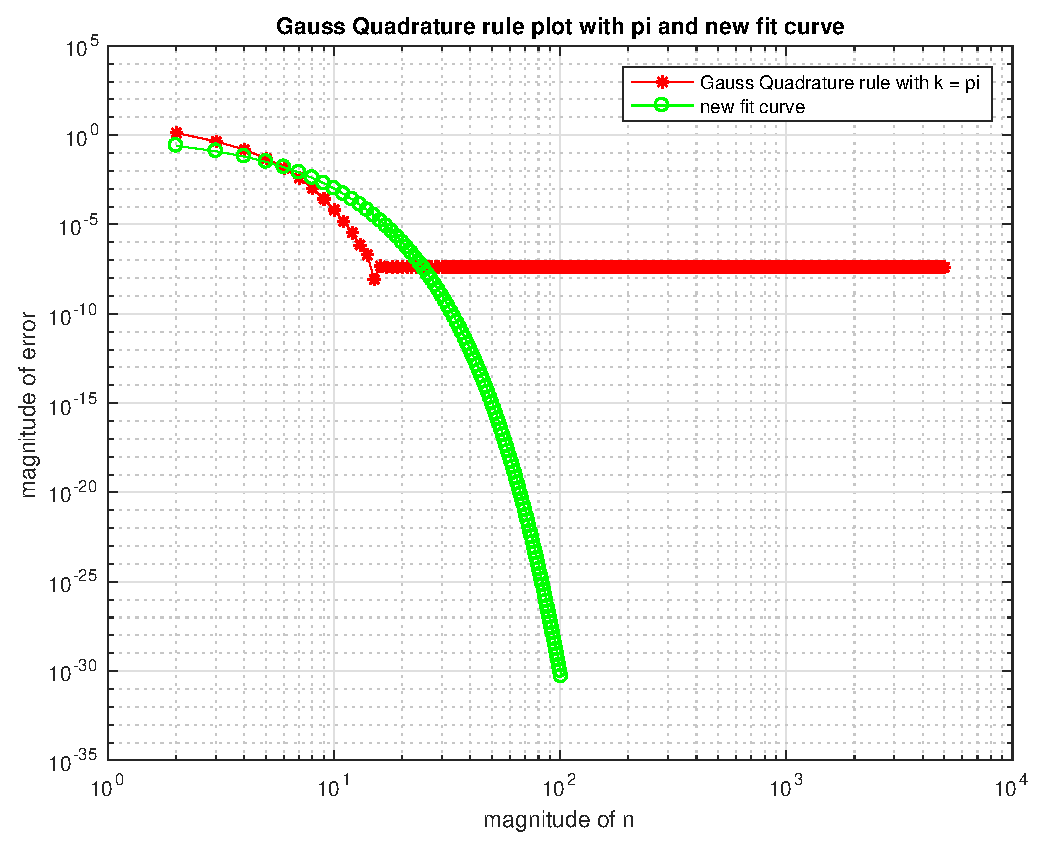
\includegraphics[width=1.0\textwidth]{Gauss_fit_1.eps}
\caption{Gauss Quadrature rule plot with k = pi and new curve (C = 1000 and a = 0.1). \label{fig:3}}
\end{center}
\end{figure} 
\begin{figure}[htb]
\begin{center}
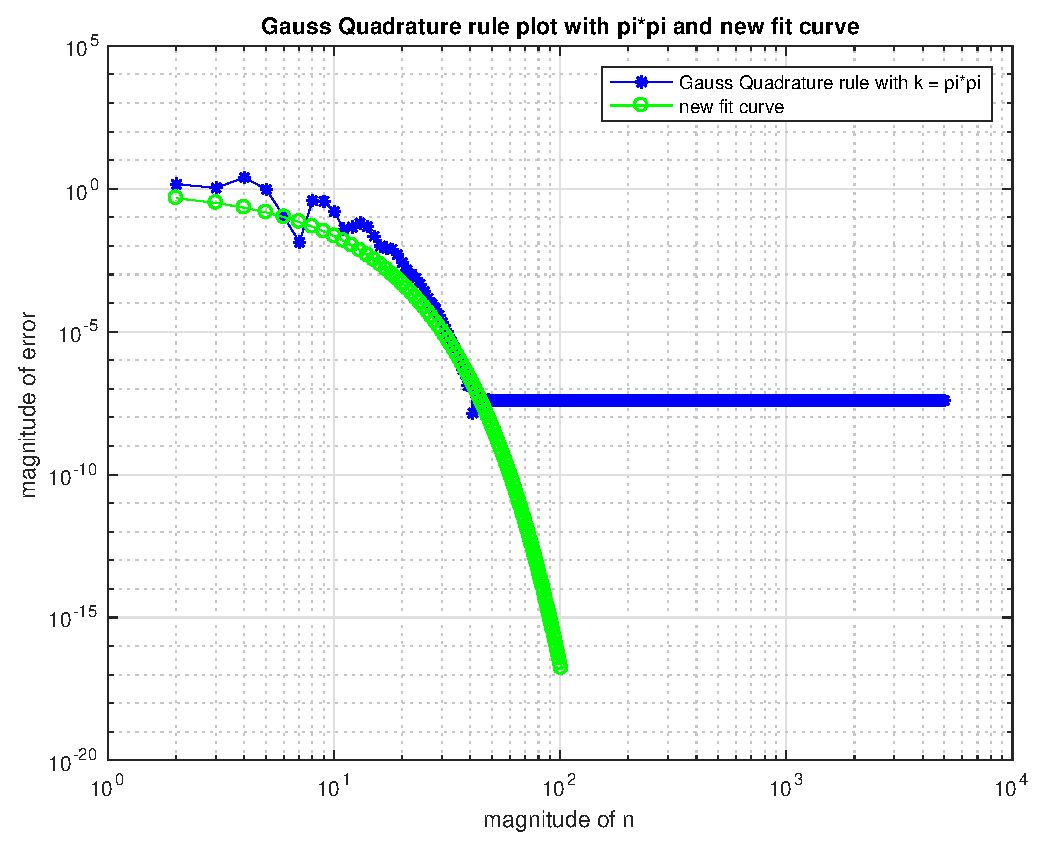
\includegraphics[width=1.0\textwidth]{Gauss_fit_2.eps}
\caption{Gauss Quadrature rule plot with k = pi*pi and new curve (C = 70 and a = 0.09). \label{fig:4}}
\end{center}
\end{figure} 

\subsection{Gauss Quadrature results discussion}
Using Gauss Quadrature, the author has the result data plot in Fig
2. It is clear that with coefficient k = pi, the data converges
faster. The author uses five thousand iterations for both k = pi and k
=pi*pi. It looks that neither of them could make the error smaller
than $10^{-10}$.
\end{document}


